%%% template.tex
%%%
%%% This LaTeX source document can be used as the basis for your technical
%%% paper or abstract. Regardless of the length of your document, the commands
%%% are all the same.
%%% 
%%% The "\documentclass" command is the first command in your file. If you want to 
%%% prepare a version of your article with line numbers - a "review" version - 
%%% include the "review" parameter:
%%%    \documentclass[review]{acmsiggraph}
%%%

\documentclass{acmsiggraph}

%%% Title of your article or abstract.

\title{Fourier Analysis of Numerical Integration in Monte Carlo Rendering:  \\Theory and Practice}

\author{
Kartic Subr  \thanks{e-mail:k.subr@hw.ac.uk}\\Heriot Watt University 
\and Wojciech Jarosz  \thanks{e-mail:wojciech.k.jarosz@dartmouth.edu}\\Dartmouth College
\and Gurprit Singh  \thanks{e-mail:gurprit.singh@dartmouth.edu}\\Dartmouth College
}
\pdfauthor{Kartic Subr}

%%% Used by the ``review'' variation; the online ID will be printed on 
%%% every page of the content.

\TOGonlineid{45678}

% User-generated keywords.

\keywords{Fourier analysis, Monte Carlo sampling, numerical integration}

% With the "\setcopyright" command the appropriate rights management text will be added
% to your document.

%\setcopyright{none}
%\setcopyright{acmcopyright}
%\setcopyright{acmlicensed}
\setcopyright{rightsretained}
%\setcopyright{usgov}
%\setcopyright{usgovmixed}
%\setcopyright{cagov}
%\setcopyright{cagovmixed}
%\setcopyright{rightsretained}

% The year of publication in the "\copyrightyear" command.

\copyrightyear{2016}

%%% Conference information, from the completed rights management form.
%%% The "\conferenceinfo" command has two parameters: 
%%%    - conference name
%%%    - conference date and location
%%% The "\isbn" field includes the year and month after the article ISBN.

\conferenceinfo{SIGGRAPH 2016 Posters}{July 24-28, 2016, Anaheim, CA} 
\isbn{978-1-4503-ABCD-E/16/07} 
\doi{http://doi.acm.org/10.1145/9999997.9999999}

\begin{document}

%%% This is the ``teaser'' command, which puts an figure, centered, below 
%%% the title and author information, and above the body of the content.

 \teaser{
   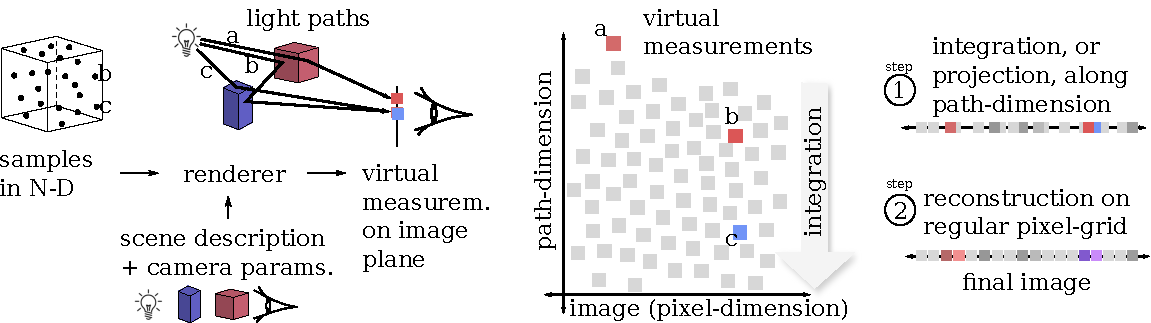
\includegraphics[height=1.6in]{../CourseNotes/Pictures/RenderHL.pdf}
   \caption{Spring Training 2009, Peoria, AZ.}
 }

\maketitle

\begin{abstract}

Since being introduced to graphics in the 1980s, Monte Carlo sampling has become the cornerstone of most modern algorithms that are used to generate high-quality, photorealistic imagery. Originally introduced to combat the effect of aliasing when estimating values at pixels, it has attained popularity as a general tool for solving complex, multi-dimensional integration problems in rendering. In this context, MC integration involves \textit{sampling} a function at various stochastically placed points and averaging the sampled values to approximate an integral, e.g. the radiance through a pixel integrated across the multi-dimensional space of possible light transport paths. Unfortunately, such estimation is error-prone and the visual manifestation of this error depends critically on the properties of the integrand, placement of the stochastic sample points used, and the type of problem (integration vs.\ reconstruction) that is being solved with these samples.

Fourier analysis, along with the Nyquist theorem, have long been used in graphics to motivate more intelligent sampling strategies which try to minimize errors due to noise and aliasing in the \textit{pixel reconstruction problem}. Only more recently, however, has the community started to apply these same Fourier tools to analyze error in the Monte Carlo \textit{integration problem}. Loosely speaking, in the context of rendering a 2D image, these two problems are concerned with errors introduced across pixels (reconstruction) vs.\ the errors introduced within any individual pixel (integration). In this course, we focus on the latter, and survey the recent developments and insights that Fourier analyses have provided about the magnitude and convergence rate of Monte Carlo integration error. We provide a historical perspective of Monte Carlo in graphics, review the necessary mathematical background, summarize the most recent developments, discuss the practical implications of these analyzes on the design of Monte Carlo rendering algorithms, and identify important remaining research problems that can propel the field forward.

\end{abstract}

%
% The code below should be generated by the tool at
% http://dl.acm.org/ccs.cfm
% Please copy and paste the code instead of the example below. 
%
\begin{CCSXML}
<ccs2012>
<concept>
<concept_id>10010147.10010371.10010372</concept_id>
<concept_desc>Computing methodologies~Rendering</concept_desc>
<concept_significance>500</concept_significance>
</concept>
<concept>
<concept_id>10010147.10010371.10010372.10010374</concept_id>
<concept_desc>Computing methodologies~Ray tracing</concept_desc>
<concept_significance>100</concept_significance>
</concept>
</ccs2012>
\end{CCSXML}

\ccsdesc[500]{Computing methodologies~Rendering}
% \ccsdesc[100]{Computing methodologies~Ray tracing}
%
% End generated code
%

% The next three commands are required, and insert the user-generated keywords, 
% The CCS concepts list, and the rights management text.
% Please make sure there is a blank line between each of these three commands.

\keywordlist

\conceptlist

\printcopyright

\section{Estimation errors due to sampling patterns}
Modern algorithms that are used to generate high-quality photorealistic pictures proceed by simulating the flow of radiant spatio-directional light energy (radiance) within environments. Given the geometric and material specifications of the objects in any scene, most \textit{renderers} output simulated images as seen through a virtual camera whose parameters are pre-specified. Such renderers essentially perform two important steps: First, they \textit{estimate} the radiance arriving at various points on the virtual sensor (of the specified camera) via simulation of light; and second, they \textit{reconstruct} the output image by resampling the estimated values on a regular grid of pixel-centers that lie on the virtual sensor. This course is dedicated to understanding errors in the former (estimation).

A popular approach for estimation proceeds by implicitly mapping high-dimensional random samples to \textit{important} light paths in the scene, followed by a carefully-weighted deposition of the radiance contributed by each path as (if) it impinges on the image plane. The efficiency of \textit {Monte Carlo renderers} can be quantified by how rapidly the image plane is populated with important estimates of radiance. The quality of the resulting estimation crucially depends on the statistical properties of the \textit {sampling pattern}, or the sum of impulses in the high-dimensional input space, which is used to generate the paths. To be practically useful, a renderer must be both efficient as well as able to generate ``high-quality'' estimation. The notion of quality, in the estimation of global illumination, is plagued by error from many sources~\cite{arvo1994framework}. 

The scope of this course will be limited to understanding approximation errors, in the estimation of numerically integrated radiance values, which stem from the choice of particular sampling patterns.

\section{Fourier analysis of estimation error}
During the process of estimation, multiple (vastly different) paths may co-incide on any given pixel. At one such pixel, imagine storing an array of \textit{all} the radiance values contributed by the paths arriving there. The histogram of this array is representative of the distribution of radiance at that pixel. The difference between the expected value of this distribution (or the average of the values in the array) and the true radiance at the pixel, \textit{bias} of the estimator, quantifies the accuracy of the simulation.  The second central moment of the distribution (or the \textit{variance} of the values in the array) quantifies the precision of the estimator. The behaviour of bias and variance at a pixel as the number of paths contributing radiance to that pixel increases is called the \textit{convergence rate}. 

In practice, errors in estimation appear in the image as coherent structured artifacts (e.g.~banding), low-frequency smears and high-frequency noise. The first two are attributed to bias, while the third is attributed to variance. Although each pixel in an image is assigned a single, averaged estimate, poor precision leads to disagreement between estimates of neighboring pixels. If these neighboring pixels lie on what should be a smooth part of the image, the disagreement manifests as noise. 

While some estimators exhibit higher error than others for a budget of (say) 10 samples per pixel, their better convergence rate could lead to dramatically superior rendering at a higher computational budget of (say) 1000 samples per pixel.~i.e.~the estimator of choice for a scene may also depend on the computational budget (interactive vs offline rendering). Recent work have derived the mean-squared error~\cite{durand2011frequency,Ramamoorthi:2012}, variance~\cite{Subr:2013:FAS,subr14error} and convergence rates~\cite{Pilleboue:2015:VAM} as functions of the Fourier statistics of sampling patterns that are popularly used in Monte Carlo rendering. A thorough understanding of error will allow informed choices potentially leading to the use of the ``best available'' sampling strategy for a given scene and computational budget. 

\section{Course objectives and overview}
  

\begin{figure*}[thbp]
  \centering
  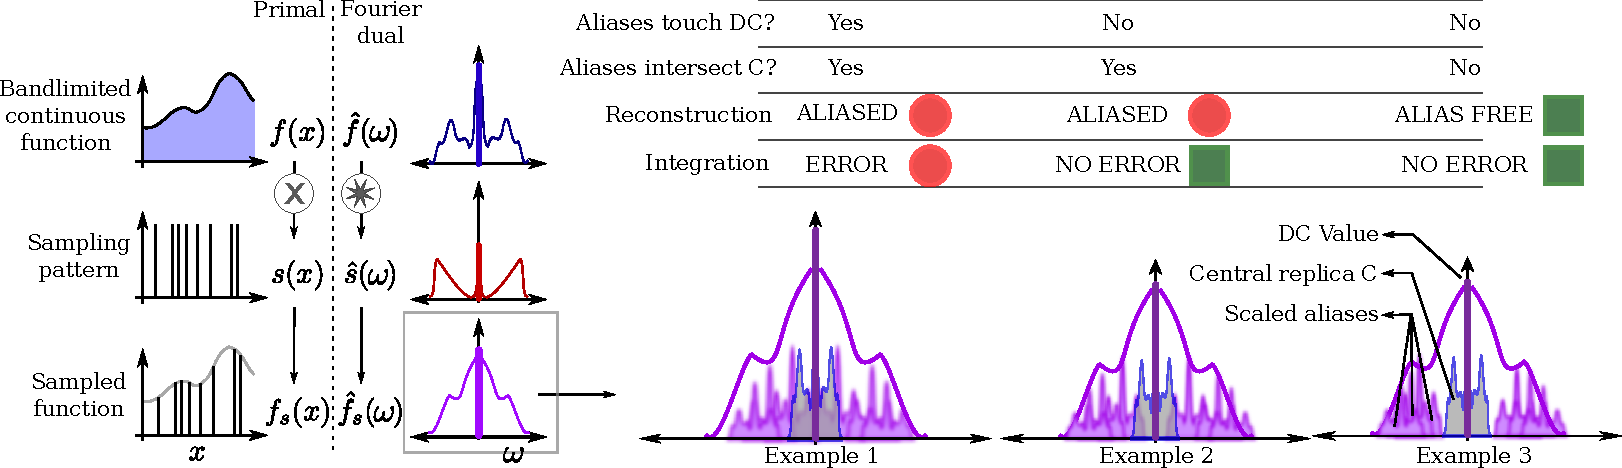
\includegraphics[width=\linewidth]{../CourseNotes/Pictures/IntegRecons.pdf}
  \caption{Ferrari LaFerrari. Image courtesy Flickr user ``gfreeman23.''}
  \label{fig:ferrari}
\end{figure*}


\section*{Acknowledgements}

\bibliographystyle{acmsiggraph}
% \nocite{*}
\bibliography{2abs}
\end{document}
